\input{../../tex_header}

\title{Chapter 21 Solusion}
\date{1/3/2022}

\begin{document}
\maketitle

\section*{21.1}

\subsection*{21.1-1}

\begin{tabular}{c|ccccccccccc}
    Edge processed & \multicolumn{11}{c}{Collection of disjoint sets} \\
    \hline
    initial sets & $\{ a \}$ & $\{ b \}$ & $\{ c \}$ & 
    $\{ d \}$ & $\{ e \}$ & $\{ f \}$ & $\{ g \}$ & 
    $\{ h \}$ & $\{ i \}$ & $\{ j \}$ & $\{ k \}$ \\
    $(d,i)$ & $\{ a \}$ & $\{ b \}$ & $\{ c \}$ & 
    $\{ d, i \}$ & $\{ e \}$ & $\{ f \}$ & $\{ g \}$ & 
    $\{ h \}$ &  & $\{ j \}$ & $\{ k \}$ \\
    $(f,k)$ & $\{ a \}$ & $\{ b \}$ & $\{ c \}$ & 
    $\{ d, i \}$ & $\{ e \}$ & $\{ f, k \}$ & $\{ g \}$ & 
    $\{ h \}$ &  & $\{ j \}$ &  \\
    $(g,i)$ & $\{ a \}$ & $\{ b \}$ & $\{ c \}$ & 
    $\{ d, g, i \}$ & $\{ e \}$ & $\{ f, k \}$ &  & 
    $\{ h \}$ &  & $\{ j \}$ &  \\
    $(b,g)$ & $\{ a \}$ & $\{ b, d, g, i \}$ & $\{ c \}$ & 
     & $\{ e \}$ & $\{ f, k \}$ &  & 
    $\{ h \}$ &  & $\{ j \}$ &  \\
    $(a,h)$ & $\{ a, h \}$ & $\{ b, d, g, i \}$ & $\{ c \}$ & 
     & $\{ e \}$ & $\{ f, k \}$ &  & 
     &  & $\{ j \}$ &  \\
    $(i,j)$ & $\{ a, h \}$ & $\{ b, d, g, i, j \}$ & $\{ c \}$ & 
     & $\{ e \}$ & $\{ f, k \}$ &  & 
     &  &  &  \\
    $(d,k)$ & $\{ a, h \}$ & $\{ b, d, f, g, i, j, k \}$ & $\{ c \}$ & 
     & $\{ e \}$ &  &  & 
     &  &  &  \\
    $(b,j)$ & $\{ a, h \}$ & $\{ b, d, f, g, i, j, k \}$ & $\{ c \}$ & 
     & $\{ e \}$ &  &  & 
     &  &  &  \\
    $(d,f)$ & $\{ a, h \}$ & $\{ b, d, f, g, i, j, k \}$ & $\{ c \}$ & 
     & $\{ e \}$ &  &  & 
     &  &  &  \\
    $(g,j)$ & $\{ a, h \}$ & $\{ b, d, f, g, i, j, k \}$ & $\{ c \}$ & 
     & $\{ e \}$ &  &  & 
     &  &  &  \\
    $(a,e)$ & $\{ a, e, h \}$ & $\{ b, d, f, g, i, j, k \}$ & $\{ c \}$ & 
     &  &  &  & 
     &  &  &  \\
\end{tabular}

\subsection*{21.1-2}

\begin{proof}
    By contents in B.4, we know that the connected components of a graph
    are the equivalence classes of vertices under the ``is reachable from'' relation.
    The collection of the disjoint sets is exactly 
    the quotient set of $G.V$ by the ``is reachable from'' relation.
    It is not hard to find out that $\proc{Connected-Components}$
    construct such the quotient set 
    since the procedure unions vertices based on all edges, 
    and edges connect two reachable vertices with the smallest length of the path
    (recall that a equivalence relation must be transitive).
    Two vertices are in the same connected component if and only if 
    they are reachable from each other.
\end{proof}

\subsection*{21.1-3}

$\proc{Find-Set}$: $2 \cdot |E|$

$\proc{Union}$: $|V| - k$

\section*{21.2}

\subsection*{21.2-1}

\begin{minted}[xleftmargin=20pt,linenos]{cpp}
struct Set
{
    Node *head;
    Node *tail;
    int size;
};

struct Node
{
    int key;
    Set *set;
    Node *next;
};

void MakeSet(Node *x)
{
    x->next = nullptr;
    x->set = new Set;// need to be freed
    x->set->head = x;
    x->set->tail = x;
    x->set->size = 1;
}

Node* FindSet(Node *x)
{
    return x->set->head;
}

void Union(Node *x, Node *y)
{
    Node *node;
    if (x->set->size < y->set->size)
    {
        Union(y, x);
    }
    else
    {
        node = y->set->head;
        x->set->size += y->set->size;
        x->set->tail->next = node;
        x->set->tail = y->set->tail;
        delete y->set;
        while (node)
        {
            node->set = x->set;
            node = node->next;
        }
    }
}
\end{minted}

\subsection*{21.2-2}

collection before line 3: 
\begin{equation*}
    \{ \{ x_{1} \}, \{ x_{2} \}, \{ x_{3} \}, \{ x_{4} \}, \{ x_{5} \}, 
    \{ x_{6} \}, \{ x_{7} \}, \{ x_{8} \}, \{ x_{9} \}, \{ x_{10} \}, 
    \{ x_{11} \}, \{ x_{12} \}, \{ x_{13} \}, \{ x_{14} \}, \{ x_{15} \}, 
    \{ x_{16} \} \}
\end{equation*}

collection before line 5: 
\begin{equation*}
    \{ \{ x_{1}, x_{2} \}, \{ x_{3}, x_{4} \}, \{ x_{5}, x_{6} \}, 
    \{ x_{7}, x_{8} \}, \{ x_{9}, x_{10} \}, 
    \{ x_{11}, x_{12} \}, \{ x_{13}, x_{14} \}, \{ x_{15}, x_{16} \} \}
\end{equation*}

collection before line 7: 
\begin{equation*}
    \{ \{ x_{1}, x_{2}, x_{3}, x_{4} \}, \{ x_{5}, x_{6}, x_{7}, x_{8} \}, 
    \{ x_{9}, x_{10}, x_{11}, x_{12} \}, \{ x_{13}, x_{14}, x_{15}, x_{16} \} \}
\end{equation*}

collection before line 8: 
\begin{equation*}
    \{ \{ x_{1}, x_{2}, x_{3}, x_{4}, x_{5}, x_{6}, x_{7}, x_{8} \}, 
    \{ x_{9}, x_{10}, x_{11}, x_{12} \}, \{ x_{13}, x_{14}, x_{15}, x_{16} \} \}
\end{equation*}

collection before line 9: 
\begin{equation*}
    \{ \{ x_{1}, x_{2}, x_{3}, x_{4}, x_{5}, x_{6}, x_{7}, x_{8} \}, 
    \{ x_{9}, x_{10}, x_{11}, x_{12}, x_{13}, x_{14}, x_{15}, x_{16} \} \}
\end{equation*}

collection before line 10: 
\begin{equation*}
    \{ \{ x_{1}, x_{2}, x_{3}, x_{4}, x_{5}, x_{6}, x_{7}, x_{8},
    x_{9}, x_{10}, x_{11}, x_{12}, x_{13}, x_{14}, x_{15}, x_{16} \} \}
\end{equation*}

Hence $\proc{Find-Set}(x_2)$ and $\proc{Find-Set}(x_11)$
return a pointer points to $x_1$.

\subsection*{21.2-3}

\begin{lemma}
    Using the linked-list representation of disjoint sets and the weighted-union heuristic,
    a sequence of $h$ $\proc{Union}$ operations on a disjoint set 
    that has never been operated $\proc{Union}$
    takes $O(h \lg h)$ time.
\end{lemma}

\begin{proof}
    We claim that, after $h$ $\proc{Union}$ operations,
    the largest set has at most $h + 1$ members. 
    Notice that the number of sets decreases by one each time $\proc{Union}$ is called.
    Suppose that we have $n$ sets in which each set contains one member in the beginning.
    After the $h$ $\proc{Union}$ operations, we have $(n - h)$ sets.
    Note that each set must contain one member.
    In order to maximize the number of members in the the largest set,
    we let $(n - h - 1)$ sets contains one member, 
    and let the remaining set contains all remaining members.
    Then the remaining set contains
    \begin{equation*}
        n - (n - h - 1) = h + 1
    \end{equation*}
    members.

    We claim that each object's pointer back to its set object 
    is updated at most $\lceil \lg h \rceil$ times
    over all the $\proc{Union}$ operations.
    Let $x$ be an arbitrary object.
    By the similar approach in the proof of Theorem 21.1,
    we know that for any $k \leq h + 1$, 
    after $x$'s pointers has been updated $\lceil \lg k \rceil$ times,
    the resulting set must have at least $k$ members.
    Since the largest set has at most $h + 1$ members,
    each object's pointer is updated at most $\lg (h + 1)$ times 
    over all the $\proc{Union}$ operations.

    We claim that there are $h$ elements have been updated their pointers 
    back to their set objects at least once.
    Consider a set contains $k$ members.
    Then within this set, there are $(k - 1)$ members have been updated their pointers 
    back to their set objects at least once
    since there must exists exactly $(k - 1)$ members updated their pointers 
    from the initial pointer to the current one.
    Let $\mathcal{S}$ be our collection of sets.
    Then after the $h$ $\proc{Union}$ operations, 
    the number of elements have been updated their pointers is
    \begin{equation*}
        \sum\limits_{A \in \mathcal{S}} (|A| - 1)
        = \sum\limits_{A \in \mathcal{S}} |A| - |\mathcal{S}|
        = n - (n - h) 
        = h
    \end{equation*}
    
    Since each object's pointer is updated at most $\lceil \lg h \rceil$ times
    and there are $h$ elements have been updated their pointers,
    we conclude $h$ $\proc{Union}$ operations on a disjoint set 
    that has never been operated $\proc{Union}$
    takes $O(h \lg h)$ time.
\end{proof}

\begin{claim}
    The amortized time of $\proc{Make-Set}$ and $\proc{Find-Set}$ is $O(1)$,
    and the amortized time of $\proc{Union}$ is $O(\lg n)$.
\end{claim}

\begin{proof}
    Suppose that we performed $h$ $\proc{Union}$ operations.
    Since $n$ $\proc{Make-Set}$ operations are performed,
    we know $(m - n - h)$ $\proc{Find-Set}$ operations are performed
    By the lemma, we know that the total actual cost of $\proc{Union}$ is $O(h \lg h)$.
    Hence the total actual cost of the sequence is 
    \begin{equation*}
        O(\underbrace{n}_{\proc{Make-Set}} + \underbrace{(m - n - h)}_{\proc{Find-Set}} + 
        \underbrace{h \lg h}_{\proc{Union}}) = O(m - h + h \lg h)
    \end{equation*}
    The total amortized cost of the sequence is
    \begin{equation*}
        O(\underbrace{n}_{\proc{Make-Set}} + \underbrace{(m - n - h)}_{\proc{Find-Set}} + 
        \underbrace{h \lg n}_{\proc{Union}}) = O(m - h + h \lg n)
    \end{equation*}
    Since $h < n$, we have showed the claim successfully.
\end{proof}

\subsection*{21.2-4}

In the $i$th $\proc{Union}$ operation,
we call $\proc{Union}(x_{i+1},x_i)$.
At this time, 
the size of set contains $x_i$ contains $i$ members,
and the size of set contains $x_{i+1}$ contains $1$ members.
Then we notice, for all $i \geq 2$,
we append the list contains $x_{i+1}$
onto the list contains $x_i$
with the weighted-union heuristic,
and this only takes $\Theta(1)$ time for each operation.
We operate $n$ times $\proc{Make-Set}$
and $(n - 1)$ times $\proc{Union}$,
so the sequence takes $\Theta(n + (n - 1)) = \Theta(n)$ time.

\subsection*{21.2-5}

\begin{minted}[xleftmargin=20pt,linenos]{cpp}
struct Node
{
    int key;
    Node *next;
    // let the tail element be the set's representative
    union
    {
        Node *tail;// for non-tail elements
        Node *head;// for the tail element
    } representative;
    int size;// only for the tail element
};

void MakeSet(Node *x)
{
    x->next = nullptr;
    x->representative.head = x;
    x->size = 1;
}

Node* FindSet(Node *x)
{
    return x->next ? x->representative.tail : x;
}

void Union(Node *x, Node *y)
{
    Node **node, *x_head, *y_head, *x_representative, *y_representative;
    if (x->representative.tail->size < y->representative.tail->size)
    {
        Union(y, x);
    }
    else
    {
        x_representative = FindSet(x);
        y_representative = FindSet(y);
        x_head = x_representative->representative.head;
        y_head = y_representative->representative.head;
        x_representative->size += y_representative->size;
        node = &y_head;
        while (*node)
        {
            (*node)->representative.tail = x_representative;
            node = &((*node)->next);
        }
        *node = x_head;
        x_representative->representative.head = y_head;
    }
}
\end{minted}

\subsection*{21.2-6}

\begin{minted}[xleftmargin=20pt,linenos]{cpp}
struct Set
{
    Node *head;
    int size;
};

struct Node
{
    int key;
    Set *set;
    Node *next;
};

void MakeSet(Node *x)
{
    x->next = nullptr;
    x->set = new Set;// need to be freed
    x->set->head = x;
    x->set->size = 1;
}

Node* FindSet(Node *x)
{
    return x->set->head;
}

void Union(Node *x, Node *y)
{
    Node **node, *x_second;
    if (x->set->size < y->set->size)
    {
        Union(y, x);
    }
    else
    {
        x->set->size += y->set->size;
        x_second = x->next;
        x->next = y->set->head;
        node = &(x->next);
        delete y->set;
        while (*node)
        {
            (*node)->set = x->set;
            node = &((*node)->next);
        }
        *node = x_second;
    }
}
\end{minted}

\section*{21.3}

\subsection*{21.3-1}

The data structure in the end (rank of each node is in the parentheses): 

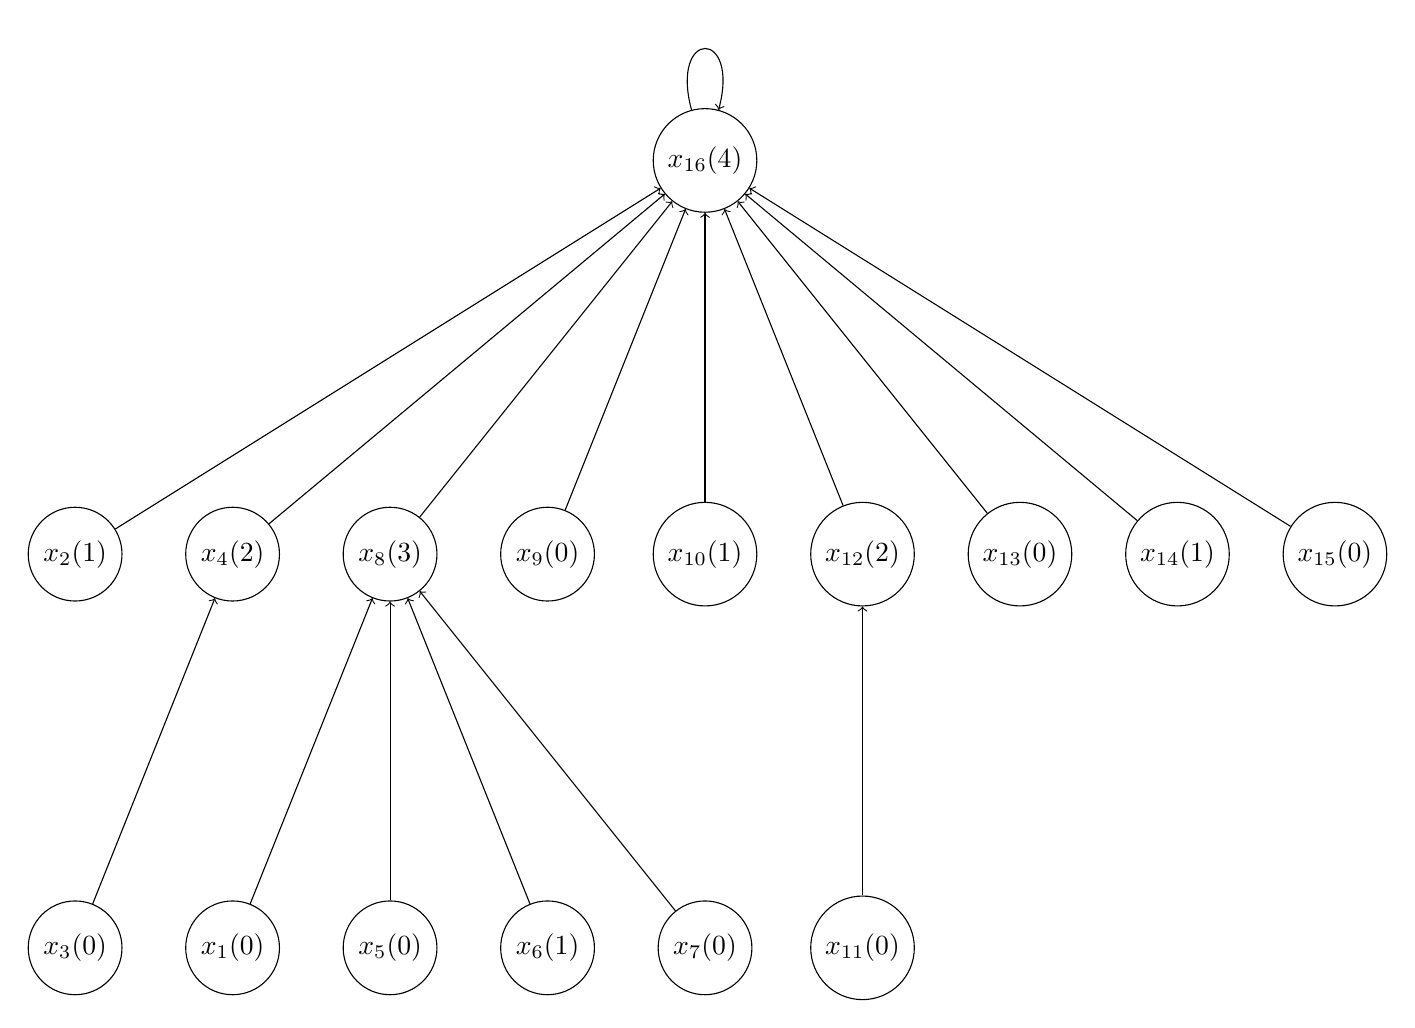
\begin{tikzpicture}
    \tikzset{vertex/.style = {shape=circle,draw,minimum size=1em}}
    \tikzset{edge/.style = {->,> = latex'}}
    \node[vertex] (x1) at (2,0) {$x_1 (0)$};
    \node[vertex] (x2) at (0,5) {$x_2 (1)$};
    \node[vertex] (x3) at (0,0) {$x_3 (0)$};
    \node[vertex] (x4) at (2,5) {$x_4 (2)$};
    \node[vertex] (x5) at (4,0) {$x_5 (0)$};
    \node[vertex] (x6) at (6,0) {$x_6 (1)$};
    \node[vertex] (x7) at (8,0) {$x_7 (0)$};
    \node[vertex] (x8) at (4,5) {$x_8 (3)$};
    \node[vertex] (x9) at (6,5) {$x_9 (0)$};
    \node[vertex] (x10) at (8,5) {$x_{10} (1)$};
    \node[vertex] (x11) at (10,0) {$x_{11} (0)$};
    \node[vertex] (x12) at (10,5) {$x_{12} (2)$};
    \node[vertex] (x13) at (12,5) {$x_{13} (0)$};
    \node[vertex] (x14) at (14,5) {$x_{14} (1)$};
    \node[vertex] (x15) at (16,5) {$x_{15} (0)$};
    \node[vertex] (x16) at (8,10) {$x_{16} (4)$};
    \draw[->] (x1) to (x8);
    \draw[->] (x2) to (x16);
    \draw[->] (x3) to (x4);
    \draw[->] (x4) to (x16);
    \draw[->] (x5) to (x8);
    \draw[->] (x6) to (x8);
    \draw[->] (x7) to (x8);
    \draw[->] (x8) to (x16);
    \draw[->] (x9) to (x16);
    \draw[->] (x10) to (x16);
    \draw[->] (x11) to (x12);
    \draw[->] (x12) to (x16);
    \draw[->] (x13) to (x16);
    \draw[->] (x14) to (x16);
    \draw[->] (x15) to (x16);
    \draw[->, loop above] (x16) to (x16);
\end{tikzpicture}

Hence $\proc{Find-Set}(x_2)$ and $\proc{Find-Set}(x_11)$
return a pointer points to $x_16$.

\subsection*{21.3-2}

\begin{minted}[xleftmargin=20pt,linenos]{cpp}
Node* FindSet(Node *x)
{
    Node *representative, *tmp;
    representative = x;
    while (representative != representative->p)
    {
        representative = representative->p;
    }
    while (x->p != representative)
    {
        tmp = x->p;
        x->p = representative;
        x = tmp;
    }
    return representative;
}
\end{minted}

\subsection*{21.3-3}

Note that we are proving that the upper bound $O(m \lg n)$ is tight (least upper bound),
instead of prove it is a tight bound $\Theta(m \lg n)$.
In order to prove it, we just need to find an example that takes $\Omega(m \lg n)$ time,
which is what the question is asking for.
We want our sequence to take as much as possible time.
WLOG, assume that $n = 2^k$ for some $k \in \NN$.
Consider the following sequence:
\begin{equation*}
\begin{split}
    \langle 
    & \proc{Make-Set}(x_1), \proc{Make-Set}(x_2), \cdots, \proc{Make-Set}(x_n), \\
    & \proc{Union}(x_1, x_2), \proc{Union}(x_3, x_4), \cdots, \proc{Union}(x_{n-1}, x_{n}), \\ 
    & \proc{Union}(x_1, x_3), \proc{Union}(x_5, x_7), \cdots, \proc{Union}(x_{n-3}, x_{n-1}), \\ 
    & \proc{Union}(x_1, x_5), \proc{Union}(x_9, x_13), \cdots, \proc{Union}(x_{n-7}, x_{n-3}), \\ 
    & \quad\quad\quad\quad\quad \vdots \\
    & \proc{Union}(x_1, x_{n / 2 + 1}), \\ 
    & \proc{Find-Set}(x_1) \cdots \quad\quad\quad \text{(until all $m$ operations are performed)} 
    \rangle
\end{split}
\end{equation*}
We performed $n$ $\proc{Make-Set}$, $(n-1)$ $\proc{Union}$, and $(m - 2n + 1)$ $\proc{Find-Set}$.
We observed we performed $n / 2$ $\proc{Union}(x_i, x_{i+1})$, $n / 4$ $\proc{Union}(x_i, x_{i+2})$,
$n / 8$ $\proc{Union}(x_i, x_{i+4})$, $\cdots$.
We conclude we performed $n / 2^j$ $\proc{Union}(x_i, x_{i+2^{j-1}})$ 
for all $j = \{ 1, 2, \cdots, \lg n \}$.
For each $j$, the height of each tree increases by $1$.
Hence after all $(n-1)$ $\proc{Union}$ operations,
the height of the tree (for the only set) is $\lg n$.
Note that $x_1$ is the deepest element in the tree.
Then, each of $\proc{Find-Set}(x_1)$ operation takes $\Theta(\lg n)$ time, 
and we perform $(m - 2n + 1)$ times $\proc{Find-Set}(x_1)$ operation.
Hence all of $\proc{Find-Set}(x_1)$ take $(m - 2n + 1)\Theta(\lg n) = \Theta(m \lg n)$ time.
We successfully find a sequence that takes $\Omega(m \lg n)$ time.

\subsection*{21.3-4}

We just need to modify $\proc{Link}$ procedure to maintain the data structure.

\begin{minted}[xleftmargin=20pt,linenos]{cpp}
void Link(Node *x, Node *y)
{
    Node *y_next;
    if (x->rank > y->rank)
    {
        y->p = x;
    }
    else
    {
        x->p = y;
        if (x->rank == y->rank)
            ++y->rank;
    }
    // maintain the circular list
    y_next = y->next;
    y->next = x->next;
    x->next = y_next;
}

std::list<Node*> PrintSet(Node *x)
{
    Node *node;
    std::list<Node*> result;
    result.push_back(x);
    for (node = x->next; node != x; node = node->next)
    {
        result.push_back(node);
    }
    return result;
}
\end{minted}

\subsection*{21.3-5}

Let $a_i$ be the number of nodes with depth greater than 0 
(i.e. non-root) in the forest after the $i$th operation.
Let $b_i$ be the number of nodes with depth greater than 1 
(i.e. non-root and non-child-of-root) in the forest after the $i$th operation.
Suppose that we start to perform $\proc{Find-Set}$ operations in the $k$th operation.
Let the potential function be
\begin{equation*}
    \Phi(D_i)
    \begin{cases}
        a_i & \text{if } i < k \text{ ,} \\
        b_i & \text{if } i \geq k \\
    \end{cases}
\end{equation*}
where $D_i$ is the disjoint forest after the $i$th operation.
Let $\Phi(D_0) = 0$.
Observed each of $\proc{Make-Set}$ and $\proc{Link}$ takes $O(1)$ time.
Denote $depth_i(x)$ as the depth of the node $x$ in the tree after the $i$th operation.
Then $\proc{Find-Set}(x)$ moves $\func{max}(0,depth_{i-1}(x) - 1)$ nodes 
to be the children of the root node.
Denote $c_i$ as the cost of the $i$th operation.
Then we assume
\begin{equation*}
    c_i = 
    \begin{cases}
        1 & \text{if $\proc{Make-Set}$ is performed in the $i$th operation,} \\
        1 & \text{if $\proc{Link}$ is performed in the $i$th operation,} \\
        \func{max}(1,depth_{i-1}(x)) & \text{if $\proc{Find-Set}(x)$ is performed in the $i$th operation} \\
    \end{cases}
\end{equation*}

\textbf{Case 1.}
$\proc{Make-Set}$ is performed in the $i$th operation.

Then $a_i = a_{i-1}$, so
\begin{equation*}
    \hat{c_i} = c_i + \Phi(D_i) - \Phi(D_{i-1})
    = 1 + 0 = 1
\end{equation*}

\textbf{Case 2.}
$\proc{Link}(x,y)$ is performed in the $i$th operation.

Note that $x$ and $y$ must be root nodes of different tree.
This operation make either $x$ or $y$ be a non-root node.
Then $a_i = a_{i-1} + 1$, so
\begin{equation*}
    \hat{c_i} = c_i + \Phi(D_i) - \Phi(D_{i-1})
    = 1 + 1 = 2
\end{equation*}

\textbf{Case 3.}
$\proc{Find-Set}(x)$ is performed in the $i$th operation.

Note that $b_i \leq a_i$ for all $i$.
If $i = k$, then 
\begin{equation*}
    \Phi(D_i) - \Phi(D_{i-1})
    = b_{i} - a_{i - 1}
    \leq b_{i} - b_{i - 1}
\end{equation*}
If $i > k$, then
\begin{equation*}
    \Phi(D_i) - \Phi(D_{i-1})
    = b_{i} - b_{i - 1}
\end{equation*}
Note that 
\begin{equation*}
    b_{i} - b_{i - 1} = - (\func{max}(1,depth_{i-1}(x)) - 1) = 1 - \func{max}(1,depth_{i-1}(x))
\end{equation*}
Hence 
\begin{equation*}
    \hat{c_i} = c_i + \Phi(D_i) - \Phi(D_{i-1})
    \leq c_i + b_{i} - b_{i - 1}
    = \func{max}(1,depth_{i-1}(x)) + (1 - \func{max}(1,depth_{i-1}(x)))
    = 1
\end{equation*}

We have shown that amortized of each operation is $O(1)$ 
with the path-compression heuristic,
no matter whether we use union by rank or not.
Hence the sequence takes $O(m)$ time 
with the path-compression heuristic,
no matter whether we use union by rank or not.

% \section*{Chapter 21 Problems}

% \subsection*{21-1}

% \subsubsection*{(a)}

\centerline{\textbf{Updating...}}

\end{document}